\documentclass[12pt]{beamer}

% ****************
% ***** INFO *****
% ****************
\usepackage[spanish]{babel}
\title[Insitute]{Trabajo final Inteligencia Artificial 1 (2024)}
\subtitle{
Visión artificial y reconocimiento de voz}
\author[Name Surname]{Name Surname}
\institute[]{Universidad Nacional de Cuyo, Facultad de Ingeniería}
\newcommand{\currentyear}{\the\year} % \currentyear
\newcommand{\nextyear}{\the\numexpr\year+1\relax} % \nextyear
\date{\currentyear/\nextyear} % or \today

% *******************
% ***** PROJECT *****
% *******************
\definecolor{main}{HTML}{0000FF}
\setbeamercolor{structure}{fg=main}

% *****************
% ***** THEME *****
% *****************
\usetheme{Madrid}
\usepackage{helvet}
\usepackage{url}
\usepackage{hyperref}
\usepackage[utf8]{inputenc} 
\renewcommand{\familydefault}{\sfdefault}
\setbeamertemplate{frametitle continuation}{\gdef\beamer@frametitle{}}
\setbeamertemplate{footline}{}

% *****************
% ***** CODE *****
% *****************
\usepackage{listings}
\lstdefinestyle{java}{
    backgroundcolor=\color{white},
    basicstyle=\ttfamily\scriptsize,
    breaklines=true,
    commentstyle=\color{gray},
    keywordstyle=\color{blue},
    stringstyle=\color{magenta},
    identifierstyle=\color{black},
    numberstyle=\color{gray},
    language=Java
}
\lstdefinestyle{cpp}{
    backgroundcolor=\color{white},
    basicstyle=\ttfamily\scriptsize,
    breaklines=true,
    commentstyle=\color{gray},
    keywordstyle=\color{blue},
    stringstyle=\color{magenta},
    identifierstyle=\color{black},
    numberstyle=\color{gray},
    language=C++
}
\lstdefinestyle{py}{
    backgroundcolor=\color{white},
    basicstyle=\ttfamily\scriptsize,
    breaklines=true,
    commentstyle=\color{gray},
    keywordstyle=\color{blue},
    stringstyle=\color{magenta},
    language=Python
}
\lstdefinestyle{js}{
    backgroundcolor=\color{white},
    basicstyle=\ttfamily\scriptsize,
    breaklines=true,
    commentstyle=\color{gray},
    keywordstyle=\color{blue},
    stringstyle=\color{magenta},
    identifierstyle=\color{black},
    numberstyle=\color{gray},
    language=JavaScript,
    escapechar=@
}
\lstdefinestyle{sh}{
    basicstyle=\ttfamily\scriptsize,
    breaklines=true,
    commentstyle=\color{gray},
    keywordstyle=\color{blue},
    stringstyle=\color{magenta},
    identifierstyle=\color{black},
    numberstyle=\color{gray},
    language=bash
}

% **********************
% ***** ALGORITHMS *****
% **********************
\usepackage{algorithm}
\usepackage{algpseudocode}

% *****************
% ***** UTILS *****
% *****************
\usepackage{xcolor}

% ********************
% ***** DOCUMENT *****
% ********************
\begin{document}

% **********************
% ***** TITLEPAGE ******
% **********************
\begin{frame}{}
\vspace{\fill}

\begin{figure}[t]
    \centering
    
\includegraphics[width=0.5\linewidth]{logofing.png}

\end{figure}

\vspace{\fill}

\Large
\color{main}
\inserttitle

\medskip

\large
\color{black}
\insertsubtitle

\vspace{\fill}

\footnotesize
\insertinstitute

\vspace{\fill}

\textbf{Autor:} Francisco Castel

\medskip

\insertdate

\vspace{\fill}
\end{frame}

% *****************
% ***** START *****
% *****************
% Diapositiva 2: Introducción
\begin{frame}{Introducción}
    \textbf{Visión Artificial}
    \begin{itemize}
        \item Identificación de objetos mediante imágenes.
        \item Aplicaciones: automatización, robótica, diagnóstico médico.
    \end{itemize}

    \vspace{0.5cm}  % Espacio entre bloques

    \textbf{Reconocimiento de Voz}
    \begin{itemize}
        \item Conversión de audio en texto o comandos.
        \item Uso de coeficientes cepstrales y modelos de clasificación.
    \end{itemize}

    \vspace{0.5cm}  % Espacio entre bloques

    \textbf{Desafíos abordados}
    \begin{itemize}
        \item Reducir dimensionalidad.
        \item Clasificación robusta en condiciones controladas.
    \end{itemize}
\end{frame}

%DIAPOSITIVA 3
\begin{frame}{Resumen}
\textbf{Objetivo}
\begin{itemize}
    \item Combinar visión artificial y reconocimiento de voz para clasificar verduras, en concreto.
    \begin{itemize}
        \item Berenjena
        \item Camote
        \item Papa
        \item Zanahoria
    \end{itemize}
\end{itemize}

\textbf{Técnicas utilizadas}
\begin{itemize}
    \item KMeans para imágenes
    \item KNN para audios
\end{itemize}

\textbf{Enfoque}
\begin{itemize}
    \item Extracción de características para cada tipo de dato
    \item Reducción de dimensionalidad para optimización y coherencia
\end{itemize}
\end{frame}


\begin{frame}{Agentes Desarrollados}
    \textbf{Clasificador de Imágenes (No Supervisado)}
    \begin{itemize}
        \item Algoritmo: \textbf{KMeans}.
        \item Características:
        \begin{itemize}
            \item Momentos de Hu.
            \item Color promedio.
        \end{itemize}
        \item Entorno controlado:
        \begin{itemize}
            \item Fondo constante.
            \item Iluminación uniforme.
        \end{itemize}
    \end{itemize}
    
    \vspace{0.5cm}  % Espacio entre bloques
\end{frame}
\begin{frame}
    \textbf{Clasificador de Audio (Supervisado)}
    \begin{itemize}
        \item Algoritmo: \textbf{KNN}.
        \item Características:
        \begin{itemize}
            \item MFCCs (media, máximo, mínimo, desviación estándar).
            \item Espectro de Potencia
            \item Entropía energética
            \item RMS y duración.
        \end{itemize}
        \item Entorno controlado:
        \begin{itemize}
            \item Bajo nivel de ruido.
        \end{itemize}
    \end{itemize}
\end{frame}

\begin{frame}{Preprocesamiento de imágenes}
    \begin{itemize}
        \item   Pasos
        \begin{enumerate}
            \item Desenfoque gaussiano
            \item Escala de grises
            \item Umbralización adaptativa
            \item Operación morfológica
        \end{enumerate}
        \item Resultados
        \begin{itemize}
            \item Mejora en la detección de contornos
            \item Reducción de ruido sal y pimienta
            \item Características finales: Momentos de Hu y color promedio
        \end{itemize}
    \end{itemize}
    
\end{frame}
\begin{frame}
\begin{table}
    \centering
    \begin{tabular}{ccc}
    
        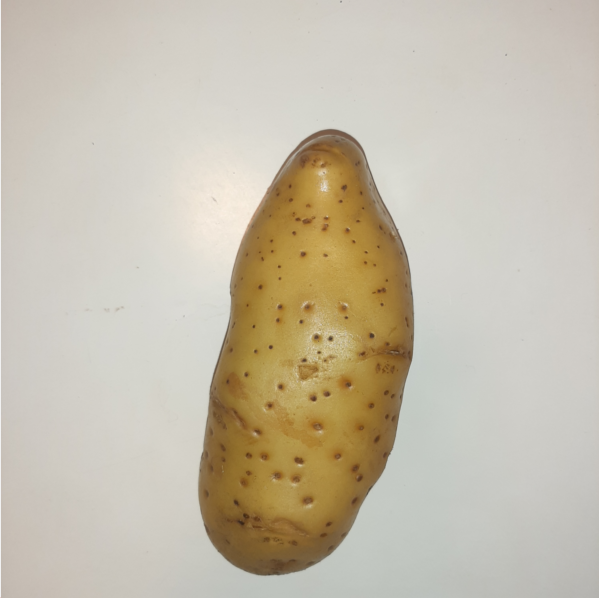
\includegraphics[width=0.25\linewidth]{gaussian.png} &
        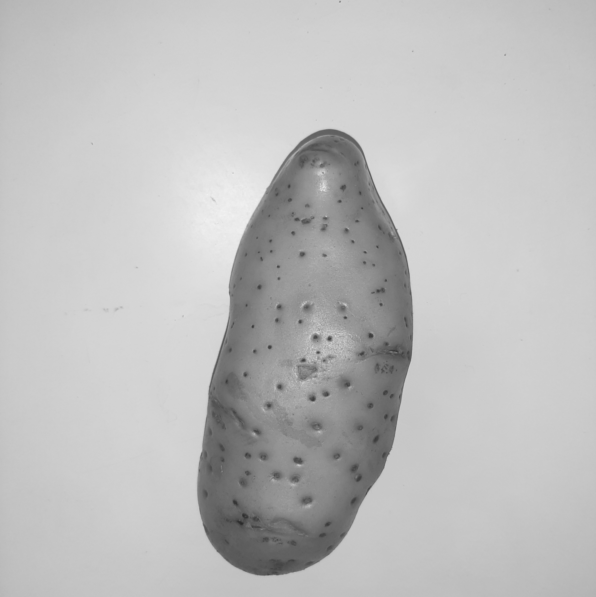
\includegraphics[width=0.25\linewidth]{gris.png}  &
        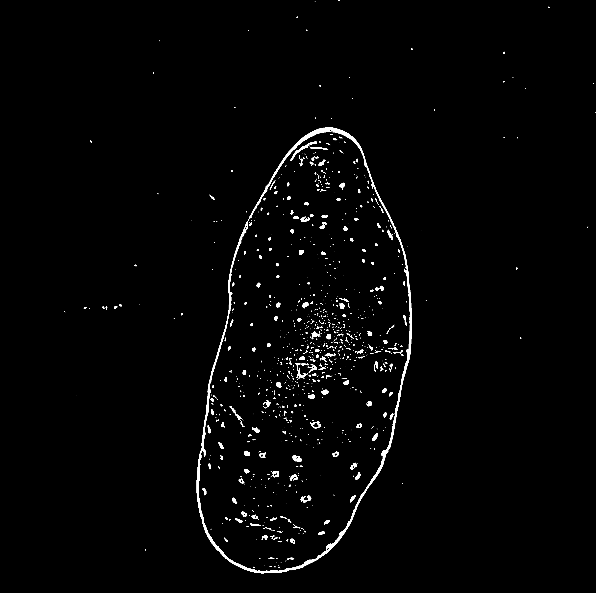
\includegraphics[width=0.25\linewidth]{binar.png} \\
        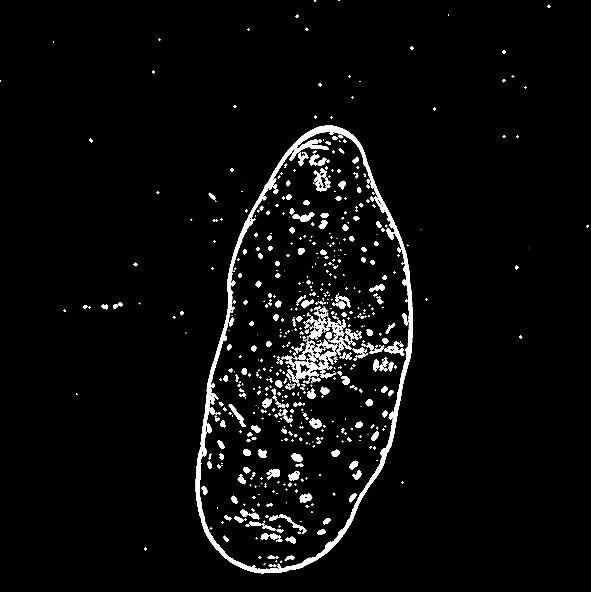
\includegraphics[width=0.25\linewidth]{morf.png} &
        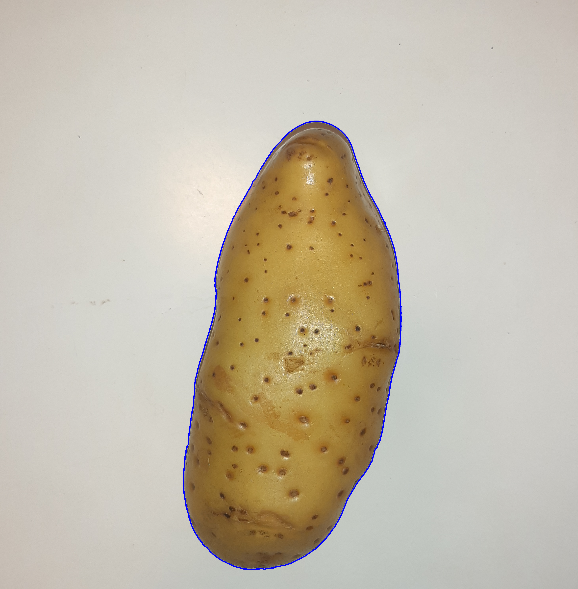
\includegraphics[width=0.25\linewidth]{contornos.png} &
        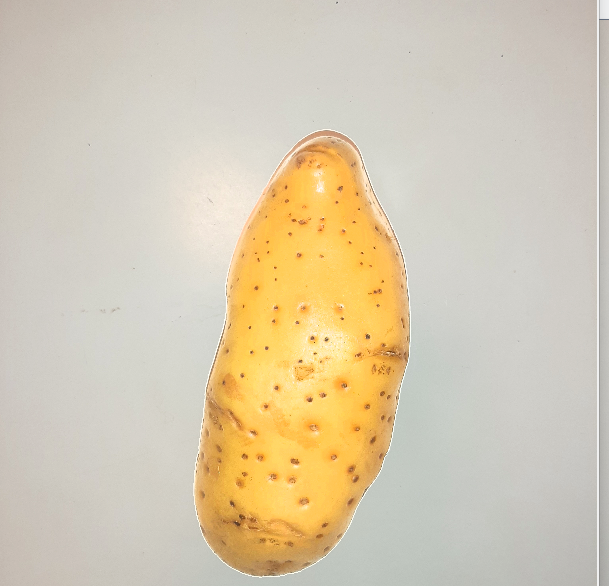
\includegraphics[width=0.25\linewidth]{mask.png} 


    \end{tabular}
    \label{tab:filtros}
\end{table}
\end{frame}

\begin{frame}{Filtro morfológico}
Consiste en dos operaciones:

\textbf{Erosión}
\vspace{0.02cm}
\begin{figure}
    \centering
    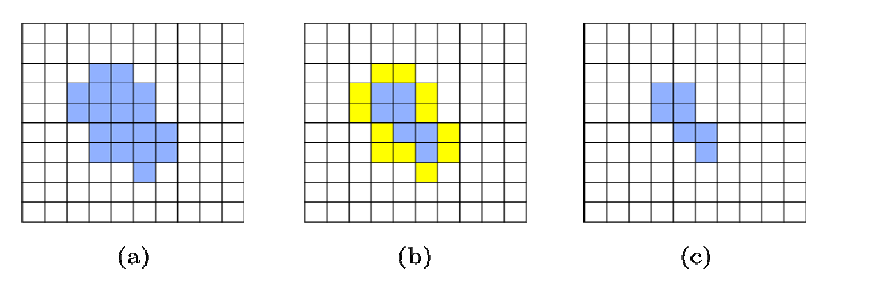
\includegraphics[width=0.6\linewidth]{erosion.png}
    
    \label{fig:erosion}
\end{figure}

\textbf{Dilatación}
\begin{figure}
    \centering
    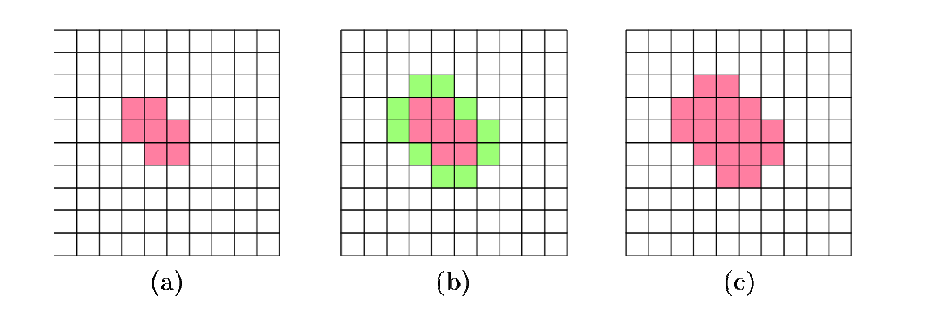
\includegraphics[width=0.6\linewidth]{dilatacion.png}
    
    
    \label{fig:dilatacion}
\end{figure}

\vspace{0.5cm}  % Espacio antes de la URL
\tiny
\url{https://riunet.upv.es/bitstream/handle/10251/145903/Ruiz\%20-\%20Aplicaci\%C3\%B3n\%20de\%20filtros\%20morfol\%C3\%B3gicos\%20en\%20im\%C3\%A1genes.pdf?sequence=1}

\end{frame}


\begin{frame}
A partir de ellas se pueden lograr dos operaciones compuestas muy interesantes.\newline
\begin{figure}
    \centering
    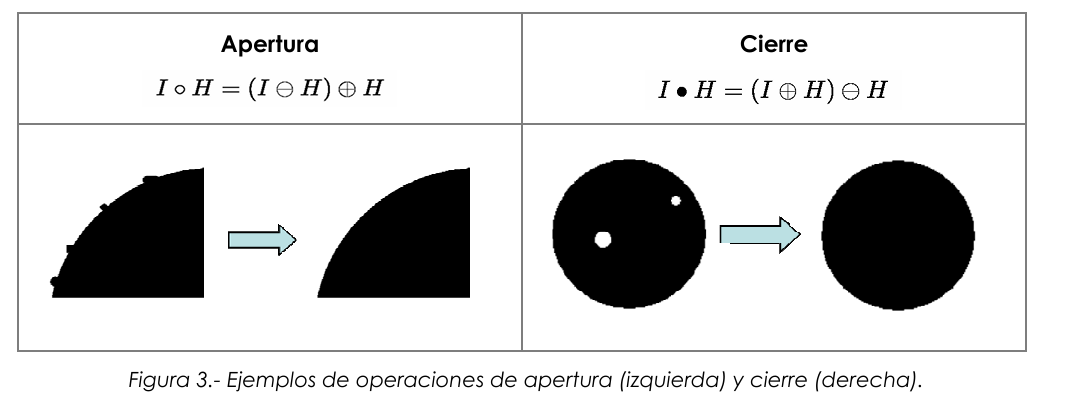
\includegraphics[width=\linewidth]{cierre.png}
    
    \label{fig:enter-label}
\end{figure}
\end{frame}

\begin{frame} {Binarización adaptativa}
La binarización adapativa es una solución práctica al inconveniente de la selección de un umbral fijo para la totalidad de la imagen. \newline
En lugar de tener un único umbral como la media de los dos valores predominantes, la media se calcula de forma local mediante una ventana definida.
\begin{table}[cc]
    \centering
    
\includegraphics[width=0.3\linewidth]{noadaptive.png}
    \hspace{0.2cm}
    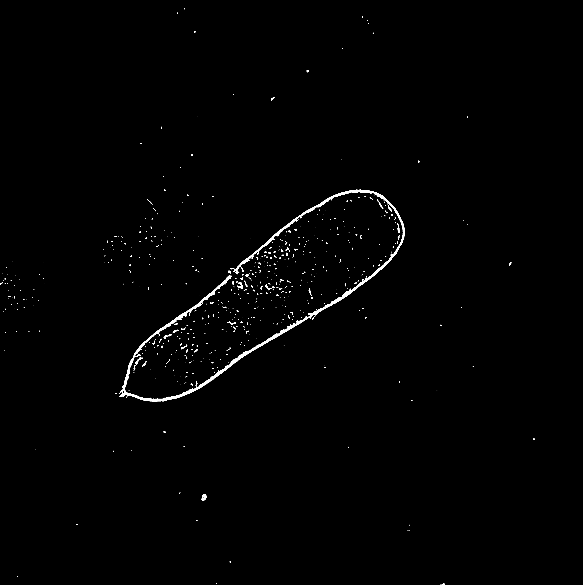
\includegraphics[width=0.3\linewidth]{adaptive.png}
    \label{tab:my_label}
\end{table}
\vspace{0.5cm}  % Espacio antes de la URL
\tiny
\url{https://www.upv.es/visor/media/0fe3f5a0-01e0-11e8-a69a-ed3f85977e27/c}
\end{frame}

\begin{frame}
\end{frame}
% ************************
% ***** BIBLIOGRAPHY *****
% ************************
\begin{frame}[allowframebreaks]{Bibliography}
Here is a reference to a source. For example, \textit{Momentum Contrast for Unsupervised Visual Representation Learning by He et al. (2020)} \cite{he2020momentum} is a placeholder text for a bibliography entry.

\framebreak

\scriptsize
\bibliographystyle{plain}
\bibliography{bib/references}
\end{frame}
% ***************
% ***** END *****
% ***************

\end{document}